\section{Введение в объектно-ориентированное программирование часть 2}
\subsection{Описание классов}
\begin{frame}[fragile]
	\frametitle{Конструкторы можно вызывать друг из друга}
	{\large Есть только одно ограничение -- вызов конструктора должен быть первый оператором.}

	\medskip
	\begin{minted}[bgcolor=bgcode,tabsize=4,linenos=true]{java}
		class Rectangle {
		    float x1, y1, x2, y2;

		    Rectangle(float ix1, float iy1,
		              float ix2, float iy2) {
		        x1 = ix1; y1 = iy1;
		        x2 = ix2; y2 = iy2;
		    }

		    Rectangle(float ix, float iy) {
		        Rectangle(0, 0, ix, iy);
		    }
		}
	\end{minted}

\end{frame}

\begin{frame}[fragile]
	\frametitle{Обычные методы тоже могут иметь одинаковые имена}

	\begin{large}
	\begin{minted}[bgcolor=bgcode,baselinestretch=0.8,linenos=true]{java}
		class Rectangle {
		    /* ... */
		    void scale(float sx, float sy) {
		        ix1 *= sx; ix2 *= sx;
		        iy1 *= sy; iy2 *= sy;
		    }

		    void scale(float s) {
		        ix1 *= s; ix2 *= s;
		        iy1 *= s; iy2 *= s;
		    }

		    /* better */
		    void scale(float s) {
		        scale(s, s);
		    }
		}
	\end{minted}
	\end{large}
\end{frame}

\begin{frame}[fragile]
	\frametitle{\textit{this} -- это ссылка на текущий объект}

	\begin{large}
	Используется для того, чтобы:
	\begin{itemize}
	\item{Передать ссылку на текущий объект в метод другого объекта}
	\item{Обратиться к полям, скрытым локальными переменными и параметрами методов}
	\end{itemize}
	\end{large}

	\begin{minted}[bgcolor=bgcode,baselinestretch=0.8,linenos=true]{java}
		class Rectangle {
		    float x1, y1, x2, y2;

		    Rectangle(float x1, float y1,
		            float x2, float y2) {
		        this.x1 = x1; this.y1 = y1;
		        this.x2 = x2; this.y2 = y2;
		    }
		
		    void testMethod(MyClass c) {
		        c.method(this);
		    }
		}
	\end{minted}
\end{frame}

\subsection{Массивы}
\begin{frame}[fragile]
	\frametitle{Массивы}

	\begin{Large}
	Объявление ссылки на массив:
	\begin{minted}[bgcolor=bgcode]{java}
	int arr[];
	Rectangle rects[];
	\end{minted}

	Создание массива:
	\begin{minted}[bgcolor=bgcode]{java}
	arr = new int[20];
	\end{minted}

	Создание массива объектов:
	\begin{minted}[bgcolor=bgcode]{java}
	rects = new Rectangle[2];
	rects[0] = new Rectangle(1, 2);
	rects[1] = new Rectangle(1, 3);
	\end{minted}
	\end{Large}
\end{frame}

\begin{frame}[fragile]
	\frametitle{Массивы}

	\begin{Large}
	Создание и заполнение массива:
	\begin{minted}[bgcolor=bgcode]{java}
	int arr[] = {1, 2, 3};
	Rectangle rects = { new Rectangle(1, 2),
	                    new Rectangle(1, 3)};
	\end{minted}

	Длина массива:
	\begin{minted}[bgcolor=bgcode]{java}
	System.out.println(rects.length);
	\end{minted}

	Работа с массивом:
	\begin{minted}[bgcolor=bgcode]{java}
	x = arr[0] + arr[1];
	for(i = 0; i < arr.length; i++)
	    System.out.println(arr[i]);
	\end{minted}

	\end{Large}
\end{frame}

\subsection{Строки}
\begin{frame}[fragile]
	\begin{Large}
	\frametitle{Строки в Java -- это объекты, а не массивы символов}

	Дополнительные возможности:
	\begin{itemize}
	\item{Создание как в языке С: \emph{\texttt{String s = "qwe";}}}
	\item{Доступен оператор \texttt{+}}
	\end{itemize}
	\medskip
	\begin{minted}[bgcolor=bgcode]{java}
	String s1 = "123";
	String s2 = "45";

	/* will print "12345" */
	System.out.println(s1 + s2);
	\end{minted}
	\end{Large}
\end{frame}

\begin{frame}[fragile]
	\frametitle{Полезные методы класса \textit{String}}

	\begin{large}
	Получить длину строки
	\begin{minted}[bgcolor=bgcode]{java}
	int length()
	\end{minted}

	Получить симовол в указанной позиции
	\begin{minted}[bgcolor=bgcode]{java}
	char charAt(int index)
	\end{minted}

	Сравнить строки (аналог функции \emph{strcmp} в С)
	\begin{minted}[bgcolor=bgcode]{java}
	int compareTo(String anotherString) 
	\end{minted}

	Сравнить строки (возвращает просто true или false)
	\begin{minted}[bgcolor=bgcode]{java}
	boolean equals(Object anObject)
	\end{minted}

	Сконвертировать в массив символов
	\begin{minted}[bgcolor=bgcode]{java}
	char[] toCharArray()
	\end{minted}
	\end{large}
\end{frame}

\begin{frame}[fragile]
	\frametitle{Полезные методы класса \textit{String}}

	\begin{large}
	Проверить, содержит ли данную последовательность символов
	\begin{minted}[bgcolor=bgcode]{java}
	boolean contains(CharSequence s)
	\end{minted}

	Разделить на части
	\begin{minted}[bgcolor=bgcode]{java}
	String[] split(String regex);
	\end{minted}

	Проверить, начинается ли строка с данной
	\begin{minted}[bgcolor=bgcode]{java}
	boolean startsWith(String prefix)
	\end{minted}

	\href{http://docs.oracle.com/javase/6/docs/api/java/lang/String.html}{документация по классу String}
	\end{large}
\end{frame}

\subsection{Работа с файлами}
\begin{frame}[fragile]
	\frametitle{Чтение байт из файла}

	\begin{Large}
	\begin{minted}[bgcolor=bgcode]{java}
	FileInputStream fis;
	byte [] buf = new byte[10];

	fis = new FileInputStream("1.txt");
	fis.read(buf);
	\end{minted}
	\end{Large}
\end{frame}

\begin{frame}[fragile]
	\frametitle{Чтение символов}

	\begin{columns}[c]
	\column{1.7in}
	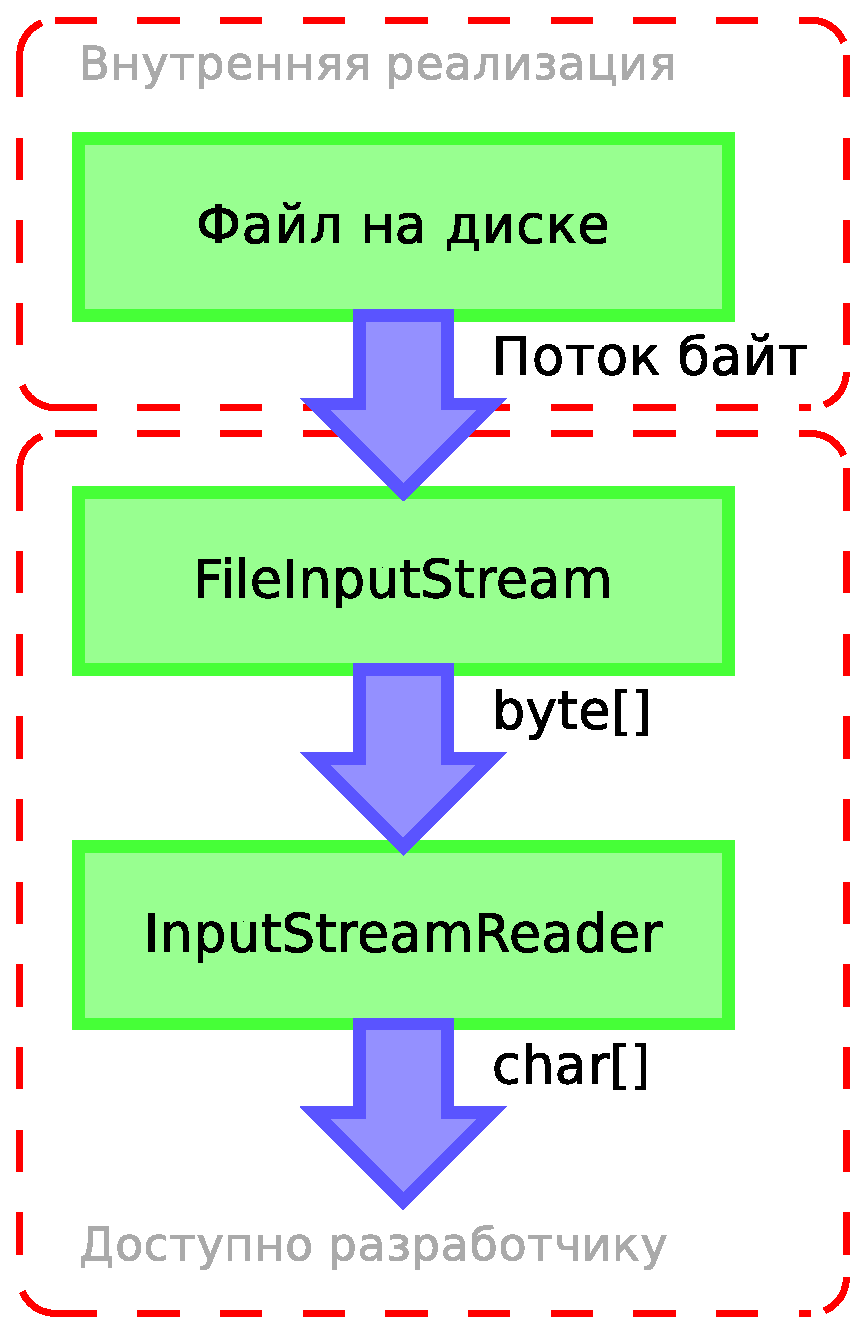
\includegraphics[width=1.8in]{lesson-3-Diagram1.eps}
	\column{2.8in}
	\begin{minted}[bgcolor=bgcode]{java}
	FileInputStream fis;
	InputStreamReader is;
	char [] buf = new char[10];

	fis = new FileInputStream("1.txt");
	is = new InputStreamReader(
	                    is, "utf-8");

	is.read(buf);
	\end{minted}
	\end{columns}
\end{frame}

\begin{frame}[fragile]
	\frametitle{FileReader -- объединение FileInputStream и InputStreamReader для удобства}

	\begin{Large}
	
	\begin{minted}[bgcolor=bgcode]{java}
	FileReader fr;
	char [] buf = new char[10];

	fr = new FileReader("1.txt");
	fr.read(buf);
	\end{minted}
	\end{Large}
\end{frame}

\subsection{Задачи}
\begin{frame}[fragile]
	\frametitle{Задачи}

	\begin{enumerate}
		\begin{item}
			Написать программу для сортировки массива случайных чисел. Напечатать массив до и после сортировки.

			Дополнения:
			\begin{itemize}
				\item{Взять размер массива из параметра командной строки, если он не указан или указано более одного параметра - напечатать справку.}
				\item{Считать массив из параметров командной строки. Размер должен определяться из числа аргументов.}
			\end{itemize}
		\end{item}
		\begin{item}
			Найти все простые числа из диапазона, заданного в командной строке 
		\end{item}
		\begin{item}
			Вычислить заданную функцию от чисел из командной строки. Реализовать функции min, max, avg, sum.


			Пример использования:
			\begin{minted}[bgcolor=bgcode]{bash}
			~: java Calc max 12 65 123 5 12 4356 42
			4356
			\end{minted}

		\end{item}

	\end{enumerate}
\end{frame}

\subsection{Полезные ресурсы}
\begin{frame}
	\frametitle{Полезные ресурсы}

	\begin{itemize}
	\item{\href{http://docs.oracle.com/javase/6/docs/}{Официальная документация}}
	\item{\href{http://www.oracle.com/technetwork/java/javase/documentation/java-se-7-doc-download-435117.html}{Архив с официальной документацией}}
	\item{\href{http://docs.oracle.com/javase/tutorial/}{Java tutorials}}
	\end{itemize}
\end{frame}

